%!TEX root = ../main.tex
\chapter{Approssimazione di derivate}

Negli scorsi capitoli siamo partiti da un problema stazionario, ovvero non dipendente dal tempo o da altre variabili indipendenti:
\begin{equation*}
\begin{cases}
-u''(x) =f(x)\\
u(0) =0\\
u(1) =0
\end{cases} \quad x\in ( 0,1)
\end{equation*}
seguendo una serie di passaggi:

\begin{figure}[htpb]
	\centering
	\tikzset{every picture/.style={line width=0.75pt}} %set default line width to 0.75pt

	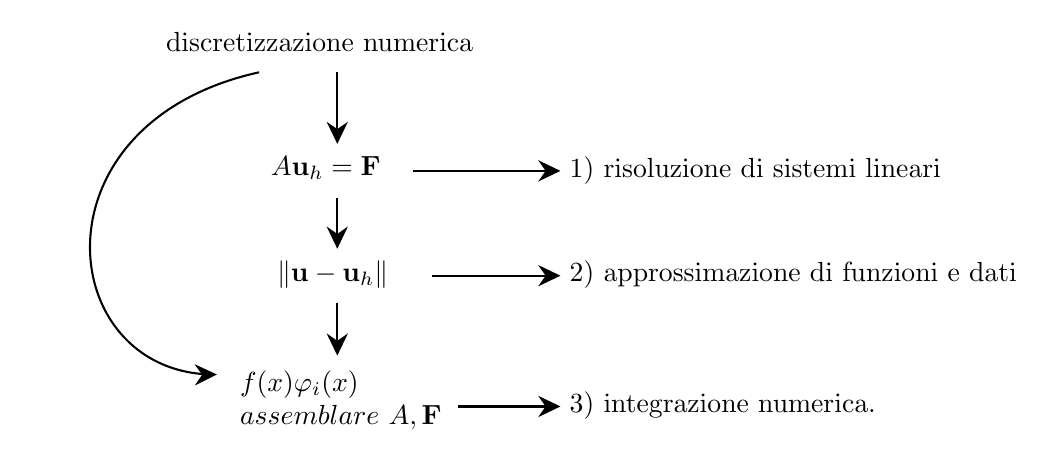
\begin{tikzpicture}[x=0.75pt,y=0.75pt,yscale=-1,xscale=1]
	%uncomment if require: \path (0,224); %set diagram left start at 0, and has height of 224


	% Text Node
	\draw (154,71.9) node [anchor=north west][inner sep=0.75pt]    {$A\mathbf{u}_{h} =\mathbf{F}$};
	% Text Node
	\draw (103.5,12) node [anchor=north west][inner sep=0.75pt]   [align=left] {discretizzazione numerica};
	% Text Node
	\draw (298,72) node [anchor=north west][inner sep=0.75pt]   [align=left] {1) risoluzione di sistemi lineari};
	% Text Node
	\draw (157,122.4) node [anchor=north west][inner sep=0.75pt]    {$\Vert \mathbf{u} -\mathbf{u}_{h}\Vert$};
	% Text Node
	\draw (298,122.5) node [anchor=north west][inner sep=0.75pt]   [align=left] {2) approssimazione di funzioni e dati};
	% Text Node
	\draw (132.5,173.9) node [anchor=north west][inner sep=0.75pt]    {$ \begin{array}{l}
	\bigintssss f(x) \varphi _{i}(x) \dx\\
	\text{assemblare} \ A,\mathbf{F}
	\end{array}$};
	% Text Node
	\draw (298,185.5) node [anchor=north west][inner sep=0.75pt]   [align=left] {3) integrazione numerica.};
	% Connection
	\draw    (187.5,33) -- (187.5,64.5) ;
	\draw [shift={(187.5,67.5)}, rotate = 270] [fill={rgb, 255:red, 0; green, 0; blue, 0 }  ][line width=0.08]  [draw opacity=0] (10.72,-5.15) -- (0,0) -- (10.72,5.15) -- (7.12,0) -- cycle    ;
	% Connection
	\draw    (187.5,93.5) -- (187.5,115) ;
	\draw [shift={(187.5,118)}, rotate = 270] [fill={rgb, 255:red, 0; green, 0; blue, 0 }  ][line width=0.08]  [draw opacity=0] (10.72,-5.15) -- (0,0) -- (10.72,5.15) -- (7.12,0) -- cycle    ;
	% Connection
	\draw    (149.81,33) .. controls (38.83,57.56) and (51.25,177.33) .. (127.18,178.61) ;
	\draw [shift={(129.5,178.61)}, rotate = 539.1600000000001] [fill={rgb, 255:red, 0; green, 0; blue, 0 }  ][line width=0.08]  [draw opacity=0] (10.72,-5.15) -- (0,0) -- (10.72,5.15) -- (7.12,0) -- cycle    ;
	% Connection
	\draw    (224,80.5) -- (292,80.5) ;
	\draw [shift={(295,80.5)}, rotate = 180] [fill={rgb, 255:red, 0; green, 0; blue, 0 }  ][line width=0.08]  [draw opacity=0] (10.72,-5.15) -- (0,0) -- (10.72,5.15) -- (7.12,0) -- cycle    ;
	% Connection
	\draw    (233,131) -- (292,131) ;
	\draw [shift={(295,131)}, rotate = 180] [fill={rgb, 255:red, 0; green, 0; blue, 0 }  ][line width=0.08]  [draw opacity=0] (10.72,-5.15) -- (0,0) -- (10.72,5.15) -- (7.12,0) -- cycle    ;
	% Connection
	\draw    (187.5,144) -- (187.5,166.5) ;
	\draw [shift={(187.5,169.5)}, rotate = 270] [fill={rgb, 255:red, 0; green, 0; blue, 0 }  ][line width=0.08]  [draw opacity=0] (10.72,-5.15) -- (0,0) -- (10.72,5.15) -- (7.12,0) -- cycle    ;
	% Connection
	\draw    (245.5,194) -- (292,194) ;
	\draw [shift={(295,194)}, rotate = 180] [fill={rgb, 255:red, 0; green, 0; blue, 0 }  ][line width=0.08]  [draw opacity=0] (10.72,-5.15) -- (0,0) -- (10.72,5.15) -- (7.12,0) -- cycle    ;

	\end{tikzpicture}
\end{figure}
\FloatBarrier

Aggiungiamo un ulteriore grado di complessità rispetto al problema proposto all'inizio del capitolo \ref{chap:introduzione}, cioè la variazione nel tempo oltre che nello spazio.
Invece di avere una corda fissata agli estremi, osserviamo una barra di metallo che riscaldiamo. Vogliamo modellizzare come varia la tempertura $u( x,t)$ in funzione dello spazio $x$ e del tempo $t$, assegnate la temperatura agli estremi, la temperatura all'istante iniziale e la sorgente termica.

Si può mostrare (ma non rientra nella nostra trattazione) che questo problema è modellato dall'\textit{equazione del calore}, abbinata ad opportune condizioni:
\begin{equation}\tag{PM}\label{eq:pm-calore}
\left\{\begin{array}{ l l l }
u_{t}( x,t) -u_{xx}( x,t) =f( x,t)  & x\in ( 0,1) ,\forall t & \text{(equazione del calore)}\\
u( 0,t) =0,\quad u( 1,t) =0 & \forall t >0 & \text{(condizioni ai limiti)}\\
u( x,0) =u_{0}(x) & \forall x\in ( a,b) & \text{(condizione iniziale).}
\end{array}\right.
\end{equation}
La funzione cercata $u( x,t)$ è la soluzione dell'equazione del calore.
Questa è un esempio di \textit{equazione differenziale}, che approfondiremo nel capitolo \ref{chap:edo}.
La risoluzione di questo tipo di equazione è uno dei principali motivi di interesse per l'approssimazione numerica di derivate.

Riscriviamo \eqref{eq:pm-calore} nel seguente modo, moltiplicando per una certa funzione $v=v(x)$ e integrando in $( 0,1)$:
\begin{equation*}
\int\nolimits ^{1}_{0}( u_{t} v-u_{xx} v) \dx=\int\nolimits ^{1}_{0} fv\dx.
\end{equation*}
Integriamo poi per parti il primo membro:
\begin{equation*}
\int\nolimits ^{1}_{0} u_{t} v\dx+\int\nolimits ^{1}_{0} u_{x} v_{x} \dx-[ u_{x} v]^{1}_{0} =\int\nolimits ^{1}_{0} fv\dx.
\end{equation*}
Come nel caso già affrontato in sezione \ref{sec:formulazione-debole}, $v$ è una funzione, in uno spazio ancora non definito, tale che $v(0) =0$, $v(1) =0$.
Si ha dunque:
\begin{equation*}
[ u_{x} v]^{1}_{0} =u_{x}( 1,t) v(1) -u_{x}( 0,t) v(0) =0.
\end{equation*}
Riscriviamo quindi il problema \eqref{eq:pm-calore}. $\forall t >0$,  trovare $u( x,t) \in V$ tale che:
\begin{equation*}\tag{PM'}\label{eq:pm1-calore}
\begin{cases}
\int\nolimits ^{1}_{0} u_{t}( x,t) v(x) \dx+\int\nolimits ^{1}_{0} u_{x}( x,t) v_{x}(x) \dx=\int\nolimits ^{1}_{0} f( x,t) v(x) \dx,\ \ \forall v\in V,\\
u( x,0) =u_{0}(x) ,
\end{cases}
\end{equation*}
dove
\begin{equation*}
V=\{
v:( 0,1)\rightarrow \mathbb{R} \ \text{tale che} \ v, v_{x} \in L^{2}( 0,1) ,\ v(0) =0,\ v(1) =0\}
\end{equation*}
è uno spazio infinito-dimensionale.
Vogliamo utilizzare invece uno spazio finito-dimensionale $V_{h} \subseteq V$, cioè tale che $\mathrm{dim}( V_{h}) =N_{h} < +\infty $.
Riscriviamo \eqref{eq:pm-calore} in $V_{h}$. $\forall t >0$ trovare $u_{h}( x,t) \in V_{h}$ tale che:
\begin{equation*}\tag{PN}\label{eq:pn-calore}
\begin{cases}
\int\nolimits ^{1}_{0}\frac{\partial u_{h}( x,t)}{\partial t} v_{h}(x) \dx+\int\nolimits ^{1}_{0}\frac{\partial u_{h}( x,t)}{\partial x}\frac{\partial v_{h}(x)}{\partial x} \dx=\int\nolimits ^{1}_{0} f( x,t) v_{h}(x) \dx,\ \ \forall v_{h} \in V_{h} ,\\
u_{h}( x,0) =u^{h}_{0}(x) ,
\end{cases}
\end{equation*}
dove $u^{h}_{0}(x) \in V_{h}$ è un'approssimazione di $u_{0}(x)$.

\textbf{Proprietà.}
\eqref{eq:pm-calore} è un sistema di equazioni differenziali del primo ordine della forma:
\begin{equation}
\begin{cases}
M\frac{\partial \mathbf{u}_{h}(t)}{\partial t} +A\mathbf{u}_{h}(t) =\mathbf{F}(t) ,\quad \forall t >0,\\
\mathbf{u}_{h}(0) =\mathbf{u}^{h}_{0} .
\end{cases}
\label{eq:sist-edp-pn}
\end{equation}


\textit{Dimostrazione.} Costruiamo una base per $V_{h}$
\begin{equation*}
V_{h} =\mathrm{span}\{\varphi _{1}(x) ,\varphi _{2}(x) ,\dotsc ,\varphi _{N_{h}}(x)\} ,
\end{equation*}
allora la soluzione $u_{h}( x,t)$ può essere scritta come combinazione lineare delle funzioni di base:
\begin{equation}
u_{h}( x,t) =\sum\limits ^{N_{h}}_{j=1} u_{j}(t) \varphi _{j}(x).
\label{eq:comb-lin-f-base}
\end{equation}
La dipendenza dal tempo è inclusa nei coefficienti $u_{j}(t)$.
Abbiamo pertanto costruito il vettore
\begin{equation*}
\mathbf{u}_{h}(t) =\begin{bmatrix}
u_{1}(t)\\
u_{2}(t)\\
\vdots \\
u_{N_{h}}(t)
\end{bmatrix} \in \mathbb{R}^{N_{h}} .
\end{equation*}
Riscriviamo (PN) utilizzando \eqref{eq:comb-lin-f-base} e otteniamo
\begin{gather*}
\int\nolimits ^{1}_{0}\frac{\partial }{\partial t}\left(\sum\limits ^{N_{h}}_{j=1} u_{j}(t) \varphi _{j}(x)\right) \varphi _{i}(x) \dx+\int\nolimits ^{1}_{0}\frac{\partial }{\partial x}\left[\sum\limits ^{N_{h}}_{j=1} u_{j}(t) \varphi _{j}(x)\right]\frac{\partial }{\partial x} \varphi _{i}(x) \dx=\\
=\int\nolimits ^{1}_{0} f( x,t) \varphi _{i}(x) \dx,\ \ \forall i=1,\dotsc ,N_{h}.
\end{gather*}
Usando la linearità e uno scambio tra derivata e integrale (possibile perché le due variabili coinvolte sono distinte), possiamo riorganizzare per ottenere:
\begin{gather*}
\sum\limits ^{N_{h}}_{j=1}\frac{\partial }{\partial t} u_{j}(t)\int\nolimits ^{1}_{0} \varphi _{j}(x) \varphi _{i}(x) \dx+\sum\limits ^{N_{h}}_{j=1} u_{j}(t)\int\nolimits ^{1}_{0}\frac{\partial }{\partial x} \varphi _{j}(x)\frac{\partial }{\partial x} \varphi _{i}(x) \dx=\\
=\int\nolimits ^{1}_{0} f( x,t) \varphi _{i}(x) \dx,\ \ \forall i=1,\dotsc ,N_{h} .
\end{gather*}
Definiamo ora la \textbf{matrice di massa}\index{matrice!di massa}
\begin{equation*}
M\in \mathbb{R}^{N_{h} \times N_{h}} ,\quad M_{ij} \coloneqq \int\nolimits ^{1}_{0} \varphi _{j}(x) \varphi _{i}(x) \dx,\quad \forall i,j=1,\dotsc ,N_{h} ,
\end{equation*}
e la matrice \textbf{matrice di rigidezza}\index{matrice!di rigidezza} (o \textit{stiffness matrix})
\begin{equation*}
A\in \mathbb{R}^{N_{h} \times N_{h}} ,\quad A_{ij} \coloneqq \int\nolimits ^{1}_{0}\frac{\partial }{\partial x} \varphi _{j}(x)\frac{\partial }{\partial x} \varphi _{i}(x) \dx,\quad \forall i,j=1,\dotsc ,N_{h} ,
\end{equation*}
quest'ultima è la stessa dell'equazione \eqref{eq:Au-F} presentata a inizio corso.
Infine definiamo il vettore
\begin{equation*}
\mathbf{F} \in \mathbb{R}^{N_{h}} ,\quad F_{i} =\int\nolimits ^{1}_{0} f( x,t) \varphi _{i}(x) \dx,\quad \forall i=1,\dotsc ,N_{h} .
\end{equation*}
Con queste definizioni possiamo riscrivere
\begin{equation*}\tag{EDO}
\begin{cases}
M\frac{\mathbf{\partial u}_{h}}{\partial t} +A\mathbf{u}_{h}(t) =\mathbf{F}(t) ,\quad \forall t >0,\\
\mathbf{u}_{h}(0) =\mathbf{u}^{h}_{0} .
\end{cases}
\end{equation*}
Per procedere alla risoluzione di questo \textit{problema non stazionario} avremo bisogno di far risolvere al calcolatore:
\begin{enumerate}
\item sistemi di EDO (Equazioni Differenziali Ordinarie),
\item sistemi di Equazioni Non Lineari.
\end{enumerate}

\section{Approssimazione di derivate}
Sia $f:[ a,b]\rightarrow \mathbb{R}$ derivabile con continuità e sia $\overline{x} \in ( a,b)$. Vogliamo approssimare $f'(\overline{x})$. Per definizione la derivata di $f$ in $\overline{x}$ è
\begin{equation*}
f'(\overline{x}) \coloneqq \lim _{h\rightarrow 0}\frac{f(\overline{x} +h) -f(\overline{x})}{h} ,
\end{equation*}
ma a livello numerico l'operazione di limite è ovviamente impossibile, e dovrà essere approssimata con $h$ piccoli.
Definiamo quindi la \textbf{differenza finita in avanti}\index{differenza finita!in avanti}:
\begin{equation}
f'(\overline{x}) \approx ( \delta _{+} f)(\overline{x}) :=\frac{f(\overline{x} +h) -f(\overline{x})}{h}.
\label{eq:diff-fin-avanti}
\end{equation}
La \textbf{differenza finita all'indietro}\index{differenza finita!all'indietro}:
\begin{equation}
f'(\overline{x}) \approx ( \delta _{-} f)(\overline{x}) :=\frac{f(\overline{x}) -f(\overline{x} -h)}{h}.
\label{eq:diff-fin-indietro}
\end{equation}
Infine, la media tra le due è detta \textbf{differenza finita centrata}\index{differenza finita!centrata}:
\begin{equation}
f'(\overline{x}) \approx ( \delta f)(\overline{x}) :=\frac{f(\overline{x} +h) -f(\overline{x} -h)}{2h}.
\label{eq:diff-fin-centrata}
\end{equation}

\begin{figure}[htpb]
	\centering
	\tikzset{every picture/.style={line width=0.75pt}} %set default line width to 0.75pt

	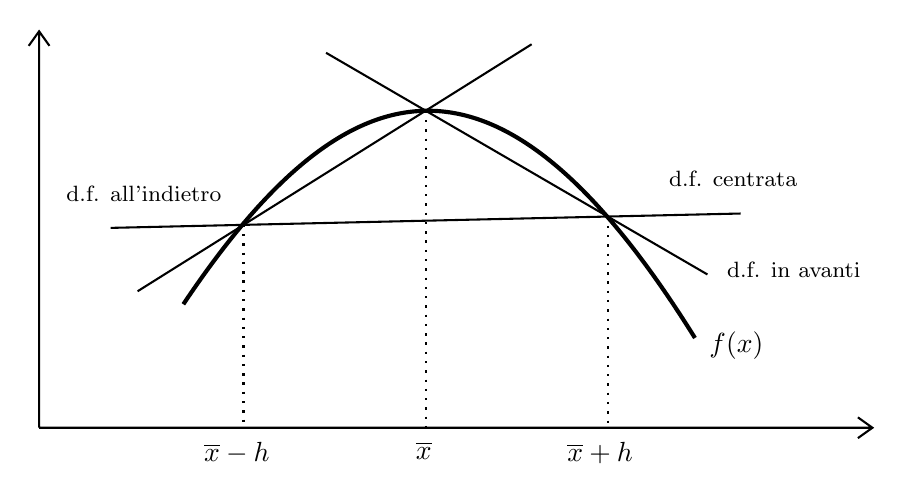
\begin{tikzpicture}[x=0.75pt,y=0.75pt,yscale=-1,xscale=1]
	%uncomment if require: \path (0,241); %set diagram left start at 0, and has height of 241

	%Shape: Axis 2D [id:dp2911281265961927]
	\draw  (116,210.5) -- (517.5,210.5)(116,19.5) -- (116,210.5) -- cycle (510.5,205.5) -- (517.5,210.5) -- (510.5,215.5) (111,26.5) -- (116,19.5) -- (121,26.5)  ;
	%Curve Lines [id:da2327769552172385]
	\draw [line width=1.5]    (185.5,151) .. controls (267,29.25) and (339.5,18.75) .. (432,167.25) ;
	%Straight Lines [id:da26722727505862176]
	\draw    (150.5,114.21) -- (454,107.29) ;
	%Straight Lines [id:da7308002840108798]
	\draw  [dash pattern={on 0.84pt off 2.51pt}]  (214.5,112.75) -- (214.5,210.5) ;
	%Straight Lines [id:da9253807449227653]
	\draw  [dash pattern={on 0.84pt off 2.51pt}]  (390,108.75) -- (390,210.5) ;
	%Straight Lines [id:da2972221464084601]
	\draw    (163.45,144.75) -- (353.3,25.75) ;
	%Straight Lines [id:da5117517681802604]
	\draw    (254.25,29.85) -- (438,136.65) ;
	%Straight Lines [id:da39389381197973306]
	\draw  [dash pattern={on 0.84pt off 2.51pt}]  (302.25,57.75) -- (302.25,210.5) ;

	% Text Node
	\draw (296,215.9) node [anchor=north west][inner sep=0.75pt]    {$\overline{x}$};
	% Text Node
	\draw (369,215.9) node [anchor=north west][inner sep=0.75pt]    {$\overline{x} +h$};
	% Text Node
	\draw (194,215.9) node [anchor=north west][inner sep=0.75pt]    {$\overline{x} -h$};
	% Text Node
	\draw (437.5,162.9) node [anchor=north west][inner sep=0.75pt]    {$f(x)$};
	% Text Node
	\draw (446,129) node [anchor=north west][inner sep=0.75pt]   [align=left] {{\footnotesize d.f. in avanti}};
	% Text Node
	\draw (127.67,92.5) node [anchor=north west][inner sep=0.75pt]  [font=\footnotesize] [align=left] {d.f. all'indietro};
	% Text Node
	\draw (418,85.5) node [anchor=north west][inner sep=0.75pt]   [align=left] {{\footnotesize d.f. centrata}};
	\end{tikzpicture}
	\caption{Intuizione grafica delle differenze all'indietro, centrate e in avanti con passo $h$.}
\end{figure}

\subsection{Errore di approssimazione delle derivate}

Supponiamo $f\in C^{2}(( a,b))$.
Possiamo sviluppare $f$ in serie di Taylor:
\begin{equation}
f(\overline{x} +h) =f(\overline{x}) +hf'(\overline{x}) +\frac{h^{2}}{2} f''( \xi ) ,\quad \xi \in (\overline{x} ,\overline{x} +h).
\label{eq:derivata-avanti}
\end{equation}
Analogamente, scrivendo l'espressione in $\overline{x} -h$:
\begin{equation}
f(\overline{x} -h) =f(\overline{x}) -hf'(\overline{x}) +\frac{h^{2}}{2} f''( \eta ) ,\quad \eta \in (\overline{x} -h,\overline{x}).
\label{eq:derivata-indietro}
\end{equation}
Possiamo riscrivere \eqref{eq:derivata-avanti} ottenendo l'errore di approssimazione:
\begin{align*}
\underbrace{\frac{f(\overline{x} +h) -f(\overline{x})}{h}}_{( \delta _{+} f)(\overline{x})} -f'(\overline{x}) & =\frac{h}{2} f''( \xi )\\
( \delta _{+} f)(\overline{x}) -f'(\overline{x}) & =\frac{h}{2} f''( \xi )\\
E^{+}(\overline{x}) & =\frac{h}{2} f''( \xi )
\end{align*}
e limitare superiormente questo errore:
\begin{align*}
 \left| E^{+}(\overline{x})\right| \leqslant \frac{h}{2}| f''( \xi )| \leqslant \frac{h}{2}\underbrace{\Vert f''(x)\Vert _{\infty }}_{\leqslant C} .
\end{align*}
Analogamente per \eqref{eq:derivata-indietro}:
\begin{align*}
\underbrace{\frac{f(\overline{x}) -f(\overline{x} -h)}{h}}_{( \delta _{-} f)(\overline{x})} -f'(\overline{x}) & =-\frac{h}{2} f''( \xi )\\
( \delta _{-} f)(\overline{x}) -f'(\overline{x}) & =-\frac{h}{2} f''( \xi )\\
E^{-}(\overline{x}) & =-\frac{h}{2} f''( \xi ) \\
\Rightarrow \ \ \left| E^{-}(\overline{x})\right| &\leqslant \frac{h}{2}| f''( \xi )| \leqslant \frac{h}{2}\underbrace{\Vert f''(x)\Vert _{\infty }}_{\leqslant C} .
\end{align*}
L'errore è quindi un infinitesimo di ordine $1$ rispetto ad $h$.

% \textit{[Lezione 16 (27-04-2020)]}

Per stimare l'errore della differenza finita centrata, supponiamo $f\in C^{3}(( a,b))$ e sviluppiamo $f$ in serie di Taylor fino all'ordine 3:
\begin{gather}
f(\overline{x} +h) =f(\overline{x}) +hf'(\overline{x}) +\frac{h^{2}}{2} f''(\overline{x}) +\frac{h^{3}}{6} f'''( \xi ) ,\quad \xi \in (\overline{x} ,\overline{x} +h) \label{eq:derivata-avanti2}\\
f(\overline{x} -h) =f(\overline{x}) -hf'(\overline{x}) +\frac{h^{2}}{2} f''(\overline{x}) -\frac{h^{3}}{6} f'''( \eta ) ,\quad \eta \in (\overline{x} -h,\overline{x}) \label{eq:derivata-indietro2}
\end{gather}
sottraiamo \eqref{eq:derivata-avanti2} e \eqref{eq:derivata-indietro2} membro a membro:
\begin{equation*}
f(\overline{x} +h) -f(\overline{x} -h) =2hf'(\overline{x}) +\frac{h^{3}}{6}[ f'''( \xi ) +f'''( \eta )].
\end{equation*}
Dividendo per $2h$:
\begin{align*}
\underbrace{\frac{f(\overline{x} +h) -f(\overline{x} -h)}{2h}}_{( \delta f)(\overline{x})} -f'(\overline{x}) & =\frac{h^{2}}{12}[ f'''( \xi ) +f'''( \eta )]\\
( \delta f)(\overline{x}) -f'(\overline{x}) & =\frac{h^{2}}{12}[ f'''( \xi ) +f'''( \eta )]\\
E(\overline{x}) & =\frac{h^{2}}{12}[ f'''( \xi ) +f'''( \eta )].
\end{align*}
Prendendo la norma infinito:
\begin{gather*}
\Vert f'''( \xi )\Vert _{\infty } \leqslant \max_{x\in ( a,b)}| f'''(x)| =:\Vert f'''(x)\Vert _{\infty } ,\\
\Vert f'''( \eta )\Vert _{\infty } \leqslant \max_{x\in ( a,b)}| f'''(x)| =:\Vert f'''(x)\Vert _{\infty } ,\\
\Rightarrow | E(\overline{x})| \leqslant \frac{h^{2}}{6}\Vert f'''(x)\Vert _{\infty } .
\end{gather*}
Abbiamo guadagnato un ulteriore ordine di infinitesimo con le differenze centrate.
Più l'ordine di infinitesimo è alto, migliore è l'approssimazione, poiché $h \ll 1$ e quindi tende a zero aumentando il suo esponente.

\textit{Osservazione.}

Supponiamo si voglia approssimare
\begin{equation*}
f'( x_{i}) ,\quad i=0,\dotsc ,n,\quad x_{i} =a+ih.
\end{equation*}
\begin{itemize}
\item Per approssimarla nei punti (nodi) interni $x_{1} \dotsc x_{n-1}$ possiamo usare le differenze finite in avanti, all'indietro o centrate, a piacere.
\item Per approssimarla in $x_{0}$ possiamo usare solo le differenze finite in avanti:
\begin{equation*}
f'( x_{0}) \approx \frac{f( x_{1}) -f( x_{2})}{h}.
\end{equation*}
\item Per approssimarla in in $x_{n}$ possiamo usare solo le differenze finite all'indietro:
\begin{equation*}
f'( x_{n}) \approx \frac{f( x_{n}) -f( x_{n-1})}{h}.
\end{equation*}
\end{itemize}

Si ha quindi meno accuratezza agli estremi.
Introducendo le \textbf{differenze finite generalizzate}\index{differenza finita!generalizzata}, facendo riferimento a sviluppi di Taylor di ordine superiore, è possibile raggiungere l'ordine di infinitesimo desiderato.

\section{Approssimazione della derivata seconda}
Sia $f\in C^{2}([ a,b])$.
Vogliamo approssimare $f''(\overline{x})$, $x\in ( a,b)$, utilizzando, come prima, gli sviluppi di Taylor.
\begin{figure}[htpb]
	\centering
	\tikzset{every picture/.style={line width=0.75pt}} %set default line width to 0.75pt

	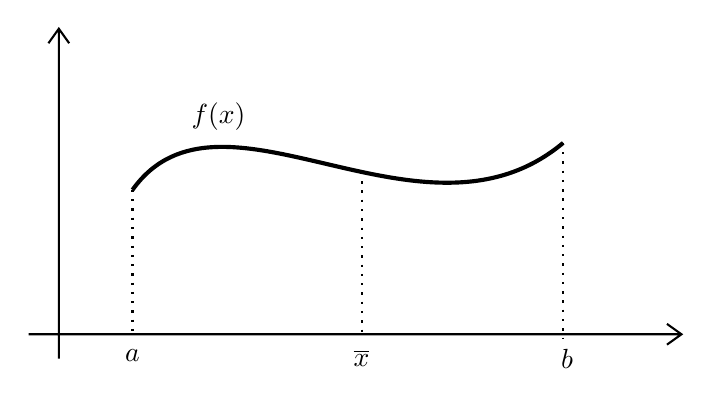
\begin{tikzpicture}[x=0.75pt,y=0.75pt,yscale=-1,xscale=1]
	%uncomment if require: \path (0,206); %set diagram left start at 0, and has height of 206

	%Shape: Axis 2D [id:dp8810490010723286]
	\draw  (141,164.56) -- (455.5,164.56)(155.5,17.34) -- (155.5,176.34) (448.5,159.56) -- (455.5,164.56) -- (448.5,169.56) (150.5,24.34) -- (155.5,17.34) -- (160.5,24.34)  ;
	%Curve Lines [id:da2795883668655186]
	\draw [line width=1.5]    (191,95) .. controls (233.5,35.34) and (330.5,129.34) .. (398.5,72.34) ;
	%Straight Lines [id:da84886858102728]
	\draw  [dash pattern={on 0.84pt off 2.51pt}]  (191,95) -- (191,165.34) ;
	%Straight Lines [id:da6214095133668482]
	\draw  [dash pattern={on 0.84pt off 2.51pt}]  (398.5,72.34) -- (398.5,166.34) ;
	%Straight Lines [id:da7636614893230751]
	\draw  [dash pattern={on 0.84pt off 2.51pt}]  (301.5,86.34) -- (301.5,165.34) ;

	% Text Node
	\draw (186,170.4) node [anchor=north west][inner sep=0.75pt]    {$a$};
	% Text Node
	\draw (396,170.4) node [anchor=north west][inner sep=0.75pt]    {$b$};
	% Text Node
	\draw (296,170.4) node [anchor=north west][inner sep=0.75pt]    {$\overline{x}$};
	% Text Node
	\draw (218,51.4) node [anchor=north west][inner sep=0.75pt]    {$f(x)$};
	\end{tikzpicture}
\end{figure}
\FloatBarrier

Fissiamo $h >0$ e scriviamo, supponendo $f\in C^{4}([ a,b])$:
\begin{gather*}
f(\overline{x} +h) =f(\overline{x}) +hf'(\overline{x}) +\frac{h^{2}}{2} f''(\overline{x}) +\frac{h^{3}}{6} f'''(\overline{x}) +\frac{h^{4}}{24} f^{\text{(iv)}}( \xi )\\
f(\overline{x} -h) =f(\overline{x}) -hf'(\overline{x}) +\frac{h^{2}}{2} f''(\overline{x}) -\frac{h^{3}}{6} f'''(\overline{x}) +\frac{h^{4}}{24} f^{\text{(iv)}}( \eta ).
\end{gather*}
con $\xi \in (\overline{x} ,\overline{x} +h)$ e $\eta \in (\overline{x} -h,\overline{x})$.
Sommiamo ora membro a membro:
\begin{equation*}
f(\overline{x} +h) +f(\overline{x} -h) =2f(\overline{x}) +h^{2} f''(\overline{x}) +\frac{h^{4}}{24}\left[ f^{\text{(iv)}}( \xi ) +f^{\text{(iv)}}( \eta )\right].
\end{equation*}
Isolando $f''(\overline{x})$:
\begin{equation*}
f''(\overline{x}) =\frac{f(\overline{x} +h) +f(\overline{x} -h) -2f(\overline{x})}{h^{2}} -\frac{h^{2}}{24}\left[ f^{\text{(iv)}}( \xi ) +f^{\text{(iv)}}( \eta )\right].
\end{equation*}
Definiamo l'approssimazione di $f''$ troncando gli infinitesimi di ordine superiore ad 1:
\begin{equation*}
f''(\overline{x}) \approx \frac{f(\overline{x} +h) +f(\overline{x} -h) -2f(\overline{x})}{h^{2}}.
\end{equation*}
L'errore di approssimazione è quindi:
\begin{equation*}
E(\overline{x}) =-\frac{h^{2}}{24}\left[ f^{\text{(iv)}}( \xi ) +f^{\text{(iv)}}( \eta )\right].
\end{equation*}
Passando alla norma infinito, otteniamo:
\begin{equation*}
| E(\overline{x})| \leqslant -\frac{h^{2}}{12}\left\Vert f^{\text{(iv)}}(x)\right\Vert _{\infty }.
\end{equation*}
Si noti che questa espressione vale solo per i nodi interni.
